\documentclass[UTF8,a4paper,12pt]{ctexart}

\usepackage[margin=2.5cm]{geometry}
\usepackage{amsmath,amssymb}
\usepackage{graphicx}
\usepackage{booktabs}
\usepackage{array}
\usepackage{caption}
\usepackage{tikz}
\usetikzlibrary{arrows.meta,positioning}
\usepackage{hyperref}

\usepackage[section]{placeins}
\usepackage{needspace}
\usepackage{float}
\renewcommand{\topfraction}{0.9}
\renewcommand{\bottomfraction}{0.8}
\renewcommand{\textfraction}{0.1}
\renewcommand{\floatpagefraction}{0.8}
\setcounter{topnumber}{3}
\setcounter{bottomnumber}{2}
\setcounter{totalnumber}{4}
\setlength{\textfloatsep}{12pt plus 2pt minus 2pt}
\setlength{\floatsep}{10pt plus 2pt minus 2pt}
\setlength{\intextsep}{10pt plus 2pt minus 2pt}
\captionsetup{font=small,skip=6pt}
\makeatletter
\setlength{\@fptop}{0pt}
\setlength{\@fpsep}{12pt plus 2pt minus 2pt}
\setlength{\@fpbot}{0pt plus 1fil}
\makeatother


% 流程图沿用结果图的蓝灰色，字号与正文一致，不缩放图中文字。
\definecolor{flowblue}{HTML}{3C5488}
\tikzset{
  flowbox/.style={draw=flowblue, fill=flowblue!4, rounded corners=2pt,
    line width=0.6pt, align=center, font=\normalsize,
    inner xsep=5pt, inner ysep=5pt},
  flownote/.style={draw=black!45, fill=black!2, align=center,
    line width=0.5pt, font=\normalsize, inner sep=5pt},
  flowarrow/.style={-{Stealth[length=2mm]}, draw=flowblue, line width=0.7pt},
  flowlabel/.style={font=\normalsize, fill=white, inner sep=2pt}
}

\graphicspath{{../figures/}}

\title{基于 Fox-Li 迭代的对称共焦腔自再现模数值研究}
\author{陈昀泽\quad U202413823\quad 光实2401}
\date{}

% 首页留白处附上仓库链接，不改变正文排版。
\AddToHookNext{shipout/foreground}{%
  \begin{tikzpicture}[remember picture,overlay]
    \node[anchor=base,inner sep=0pt,text=flowblue,
      font=\fontsize{9}{11}\selectfont]
      at ([yshift=-202bp]current page.north)
      {\href{https://github.com/CYZice/Fox-Li}{GitHub: https://github.com/CYZice/Fox-Li}};
  \end{tikzpicture}%
}

\begin{document}

\maketitle

\begin{abstract}
本文采用 Fox--Li 迭代法计算有限孔径对称共焦腔的自再现模。
根据近轴衍射积分建立一维场模型，进一步利用共焦腔积分核建立二维场模型，
通过迭代收敛性分析及理论基模对比验证数值结果，得到镜面处的数值 \(1/e\) 振幅半径约为 \(5.8\lambda\)
，与理论值 \(5.642\lambda\) 较接近，二维中心截线也与一维结果一致。

接着研究反射镜倾斜对自再现模的影响。
小角度下光束中心随倾角近似线性移动，拟合斜率约为 \(-99.9888\lambda/\mathrm{rad}\)，
与理论\(y_c\approx-L\theta\) 一致；随着正倾角增大，
倾斜方向的模半径逐渐减小，完整二维往返衍射损耗明显增加。

进一步研究镜面局部凸起对自再现模的影响，观察到环状节点和模场畸变；半径增大时附加损耗增大，
凸起移出光斑主区后影响减弱。
\end{abstract}

\noindent\textbf{关键词：} Fox--Li 迭代；光学谐振腔；自再现模式；对称共焦腔；镜面倾斜；半球凸起

\newpage
\begingroup\small\tableofcontents\endgroup
\newpage

\section{物理模型建立}

\subsection{对称共焦腔的物理模型与光场传播方程}
研究对象为两面相同球面反射镜构成的理想对称共焦腔。设腔长为 \(L\)，
两镜曲率半径均为 \(R=L\)，镜面横向坐标分别为 \((x',y')\) 和
 \((x,y)\)。采用衍射理论描述腔内光场的传播，假设光场满足近轴近似条件。

根据菲涅耳--基尔霍夫衍射积分，光场经过一次渡越后在另
一镜面上的分布为~\cite{xia2016laser,fox1961resonant}
\begin{equation}
 u_2(x,y)=\frac{\mathrm{i}k}{2\pi L}\iint_S u_1(x',y')\exp(-\mathrm{i}k\rho)\,\mathrm dx'\mathrm dy',
\end{equation}
其中，\(k=2\pi/\lambda\)，\(S\) 为镜面有效孔径，\(\rho\) 为两镜面上对应两点之间的距离。对于对称共焦腔，考虑球面镜的几何关系，在近轴近似下有
\begin{equation}
\begin{aligned}
 \rho&=L+\frac{(x-x')^2+(y-y')^2}{2L}
 -\frac{x^2+y^2+x'^2+y'^2}{2L}\\
 &=L-\frac{xx'+yy'}{L}.
\end{aligned}
\end{equation}
代入衍射积分公式，可得共焦腔的光场传播方程：
\begin{equation}\label{eq:propagation}
 u_2(x,y)=\frac{\mathrm{i}e^{-\mathrm{i}kL}}{\lambda L}
 \iint_S u_1(x',y')e^{\mathrm{i}k(xx'+yy')/L}\,\mathrm dx'\mathrm dy'.
\end{equation}
当光场经过多次渡越后，其横向分布保持不变，
仅存在整体振幅衰减和相位偏移，即形成自再现模。
设其场分布为 \(v(x,y)\)，式~\eqref{eq:propagation}对应的积分核用\(\mathcal K\) 表示
。则满足
\begin{equation}
 v(x,y)=\gamma\iint_S\mathcal K(x,y;x',y')v(x',y')\,\mathrm dx'\mathrm dy',
\end{equation}
通过 Fox--Li 迭代，可以得到自再现模的振幅、相位及衍射损耗等特性~\cite{fox1961resonant}。

\subsection{镜面扰动模型}
在理想共焦腔的基础上，进一步分析某个镜面发生扰动情况的自再现模式，
将镜面偏差作为附加相位引入反射过程。设镜面相
对于理想球面的高度偏差为 \(h(x,y)\)，正方向指向腔内。在近轴反射
的局部相位近似下，附加光程为 \(\Delta\rho\approx-2h(x,y)\)，对应的
反射相位因子为
\begin{equation}\label{eq:mirror-phase}
 M(x,y)=e^{\mathrm{i}2kh(x,y)}.
\end{equation}
对于镜面扰动模型，采用完整往返后的场分布建立
自再现条件：光场从正常镜传播到扰动镜，乘以 \(M\)，再传播回正常镜。

\subsubsection{反射镜倾斜}
设其中一面反射镜绕 \(x\) 轴倾斜小角度 \(\theta\)。小角度下，镜面高度偏差 \(h_{\mathrm{tilt}}\approx\theta y\)，由此得到
\begin{equation}
 M_{\mathrm{tilt}}(x,y)=e^{\mathrm{i}2k\theta y}.
\end{equation}
该相位沿 \(y\) 方向线性变化。

\subsubsection{镜面局部半球凸起}
设其中一面反射镜上凸起中心位置为 \((x_c,y_c)\)，半球半径为 \(r_b\)，则镜面高度偏差为
\begin{equation}\label{eq:hemisphere}
 h_{\mathrm{bump}}(x,y)=
 \begin{cases}
 \sqrt{r_b^2-(x-x_c)^2-(y-y_c)^2},&(x-x_c)^2+(y-y_c)^2\le r_b^2,\\
 0,&\text{其他区域}.
 \end{cases}
\end{equation}
对应的附加相位因子为
\begin{equation}
 M_{\mathrm{bump}}(x,y)=e^{\mathrm{i}2kh_{\mathrm{bump}}(x,y)}.
\end{equation}

\section{数值方法与程序设计}

\subsection{参数与离散网格}
数值计算以波长 \(\lambda\) 为单位一，
程序取 \(\lambda=1\)、\(k=2\pi\)。
\begin{table}[!htbp]
 \centering
 \caption{正式计算的主要参数}\label{tab:parameters}
 \begin{tabular}{ll}\toprule
 参数 & 数值\\\midrule
 腔长与主镜曲率半径 & \(L=R=100\lambda\)\\
 镜面有效孔径 & \(x,y\in[-10\lambda,10\lambda]\)，方形区域\\
 一维与二维网格 & 101 点；\(101\times101\)\\
 网格间距 & \(\Delta x=\Delta y=0.2\lambda\)\\
 默认初始场 & 均匀复振幅\\
 残差阈值与连续次数 & \(10^{-4}\)，连续 10 次\\
 \bottomrule\end{tabular}
\end{table}

\subsection{一维与二维积分}
将式~\eqref{eq:propagation} 转化为离散情况，
连续积分换成有限求和。
传播核取为
\begin{equation}\label{eq:kernel-1d}
 K_{ji}=\sqrt{\frac{\mathrm{i}}{\lambda L}}e^{-\mathrm{i}kL/2}
 e^{\mathrm{i}kx_jx_i/L}\Delta x.
\end{equation}
采样点的复振幅 \(u=(u_i)\)，一次一维传播得
\begin{equation}\label{eq:propagation-1d}
 u'_j=\sum_iK_{ji}u_i,\qquad u'=Ku.
\end{equation}

二维情形将式~\eqref{eq:propagation} 转化为离散网格情况
，取 \(U_{jl}=U(y_j,x_l)\)，得
\begin{equation}\label{eq:double-sum}
 U'_{jl}=\frac{\mathrm{i}e^{-\mathrm{i}kL}}{\lambda L}
 \sum_i\sum_m U_{im}e^{\mathrm{i}k(y_jy_i+x_lx_m)/L}\Delta x\Delta y.
\end{equation}
二维传播核在两个横向坐标上具有可分离性，
因此二维传播核可复用一维传播核
\begin{equation}\label{eq:matrix-propagation}
 U'_{jl}=\sum_i\sum_m K_{ji}U_{im}K_{lm},
 \qquad U'=KUK^{\mathrm T}.
\end{equation}

\subsection{Fox--Li 迭代、本征值与收敛判断}
从均匀初始场出发，迭代寻找自再现模式~\cite{fox1961resonant}。
以一维为例，设第 \(n\) 轮输入场为 \(u_n\)，则每轮计算为
\begin{equation}
 \widetilde u_{n+1}=Ku_n,\qquad
 u_{n+1}=\frac{\widetilde u_{n+1}}{\max_j|\widetilde u_{n+1,j}|}.
\end{equation}
其中，\(u_{n+1}\) 为每次迭代计算完毕对场分布进行归一化后的结果，再作为初始条件代入下一个循环~\cite{xia2016laser}。

若光场已接近自再现模式，传播前后的场应满足
 \(u_n\approx\gamma_n\widetilde u_{n+1}\)，
只相差一个与坐标无关的复常数。
传播后的振幅比例为 \(1/|\gamma_n|\)，
整体相位变化为 \(-\arg\gamma_n\)。

最开始我直接在传播结果非零的采样点计算 \(u_{n,j}/\widetilde u_{n+1,j}\)，
再取平均来估计 \(\gamma_n\)，
但早期计算中发现，场型已基本稳定，逐点平均得到的比例仍有明显波动。
在弱场位置，分母很小，微小的数值误差就可能造成较大的比值偏差；
在节点处，分母为零，无法直接相除。
直接平均又使弱场点与主要光场区域具有相同权重
，因此少数异常比值可能影响整体估计。

针对这一问题，本文改用整体最小二乘估计：不再分别求各点的比值，而是寻找一个共同的本征值 \(\gamma_n\)，使传播后的整个场尽可能接近 \(u_n/\gamma_n\)。对应的最优化问题为
\begin{equation}
 \min_{\gamma_n\ne0}J(\gamma_n),\qquad
 J(\gamma_n)=\sum_j\left|\widetilde u_{n+1,j}-\frac{u_{n,j}}{\gamma_n}\right|^2.
\end{equation}
将 \(1/\gamma_n\) 作为待拟合的整体传播比例，得到
\begin{equation}\label{eq:gamma}
 \gamma_n=\frac{\sum_j|u_{n,j}|^2}
 {\sum_j u_{n,j}^*\widetilde u_{n+1,j}}
 =\frac{\langle u_n,u_n\rangle}{\langle u_n,\widetilde u_{n+1}\rangle}.
\end{equation}

得到最佳整体比例后，用相对残差检验自再现条件~\cite{xia2016laser}：
\begin{equation}
 \epsilon_n=\frac{\|\widetilde u_{n+1}-u_n/\gamma_n\|_2}
 {\|\widetilde u_{n+1}\|_2}.
\end{equation}
残差越小，说明传播前后的场越接近仅相差整体比例。本文取残差连续 10 次小于 \(10^{-4}\) 为停止条件，并对最终保存场重新评估本征比例和残差。

二维计算沿用同样的比例估计、归一化和残差判据，只将单程传播改为 \(\widetilde U_{n+1}=KU_nK^{\mathrm T}\)，内积改为对全部网格点求和。对于镜面扰动，每轮则改为完整往返。记 \(P(U)=KUK^{\mathrm T}\) 为一次二维传播，\(M\) 为第 1 章定义的反射相位因子，\(A\) 为完整往返传播，则
\begin{equation}\label{eq:round-trip}
 \widetilde U_{n+1}=A(U_n)=P\bigl(M\cdot P(U_n)\bigr),
\end{equation}
其中 \(M\cdot P(U_n)\) 表示逐点乘以反射相位。此时用 \(\gamma_{\mathrm{rt}}\) 表示往返本征值，满足 \(U\approx\gamma_{\mathrm{rt}}A(U)\)，与基础计算的单程本征值区分。流程图中用 \(V\) 简记尚未归一化的传播结果，\(\mathcal T\) 表示上述单程或完整往返传播算子。基础二维独立判断收敛；可分离倾斜扫描的每方向阈值取 \(10^{-4}/\sqrt2\)，合成场仍检查二维残差。完整流程见图~\ref{fig:fox-li-flow}。
\begin{figure}[!htbp]
 \centering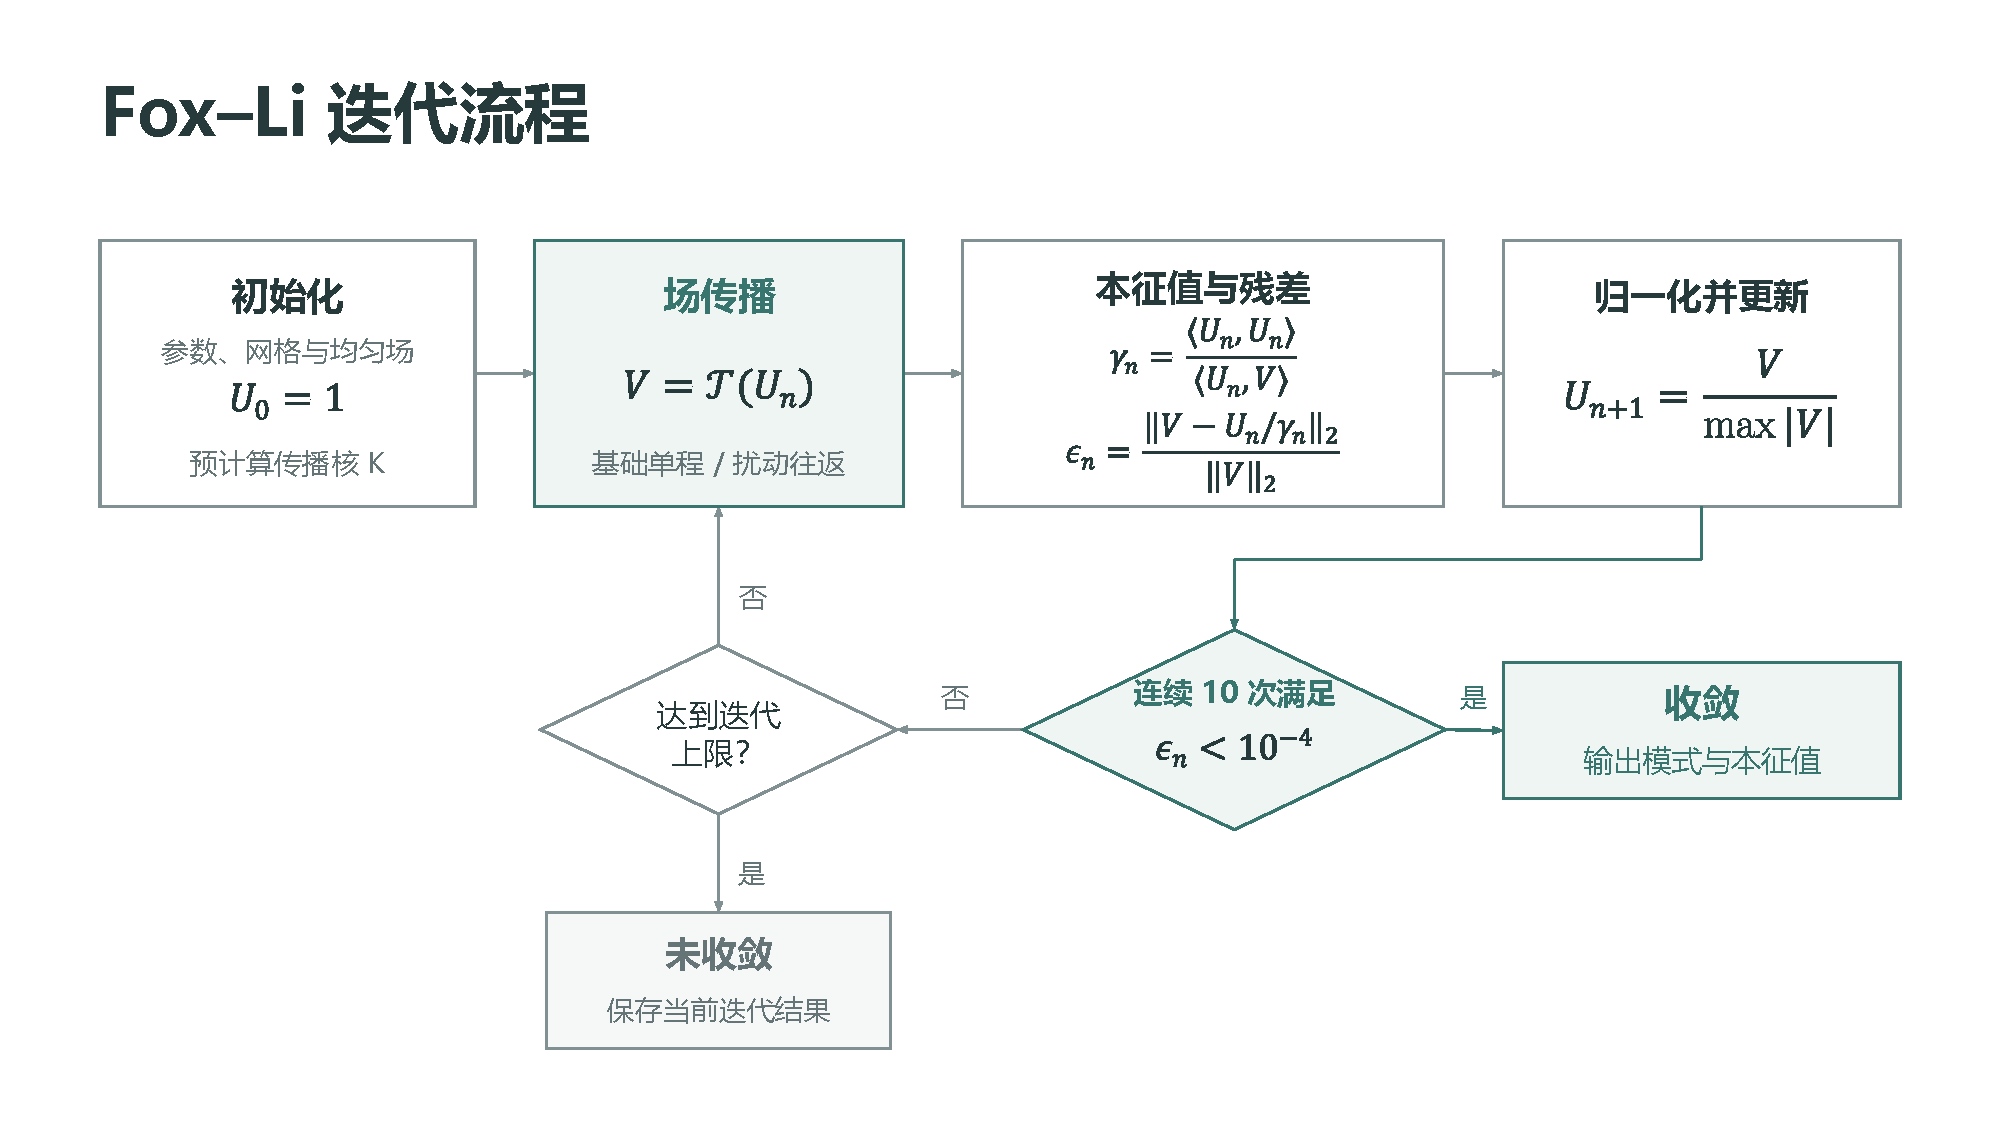
\includegraphics[width=\linewidth,trim=38bp 20bp 38bp 20bp,clip]{report_fox_li_flow.pdf}
 \caption{Fox--Li 迭代与单程、完整往返计算的对应}\label{fig:fox-li-flow}
\end{figure}

\FloatBarrier
\subsection{定量指标与损耗口径}
以 \(I_{jl}=|U_{jl}|^2\) 定义光束中心和二阶矩半径，例如
\begin{equation}
 \bar y=\frac{\sum_{j,l}y_j I_{jl}}{\sum_{j,l}I_{jl}},\qquad
 w_y=2\sqrt{\frac{\sum_{j,l}(y_j-\bar y)^2I_{jl}}{\sum_{j,l}I_{jl}}}.
\end{equation}
\(\bar x,w_x\) 同理；一维时只沿相应坐标求和。倾斜分析中 \(y_c=\bar y\)。对理想 Gaussian 强度 \(I\propto e^{-2y^2/w^2}\)，二阶矩定义给出 \(w_y=w\)，与 Gaussian 模半径对应~\cite{kogelnik1966laser}。

两种扰动统一采用完整二维往返本征值与功率损耗：
\begin{equation}\label{eq:loss}
 D=1-\frac{1}{|\gamma_{\mathrm{rt}}|^2},\qquad \Delta D=D-D_0.
\end{equation}
其中 \(D_0\) 为无扰动完整往返场的功率损耗。

模式重叠度定义为
\begin{equation}
 F=\frac{|\langle U_0,U\rangle|^2}{\|U_0\|_2^2\|U\|_2^2}.
\end{equation}
它描述模式偏离无扰动参考场的程度。

\subsection{传播核预计算}
网格和腔参数固定时，传播核不随迭代改变。程序将原离散公式的核预计算一次，后续使用矩阵乘法，减少重复求指数的开销。

\section{基础模式验证}

\subsection{一维振幅、相位与 Gaussian 理论对比}
从均匀初始场出发进行 Fox--Li 迭代后，数值场逐渐形成中心单峰、左右对称的稳定分布。图~\ref{fig:base-validation}(a) 给出一维归一化振幅与 Gaussian 理论解，(b) 给出以中心相位为参考的相对相位 \(\phi(x)-\phi(0)\)，(c) 比较一维结果与二维中心截线。相对相位沿横向坐标近似均匀，与基模的相位特征一致。

\begin{figure}[!htbp]
  \centering
  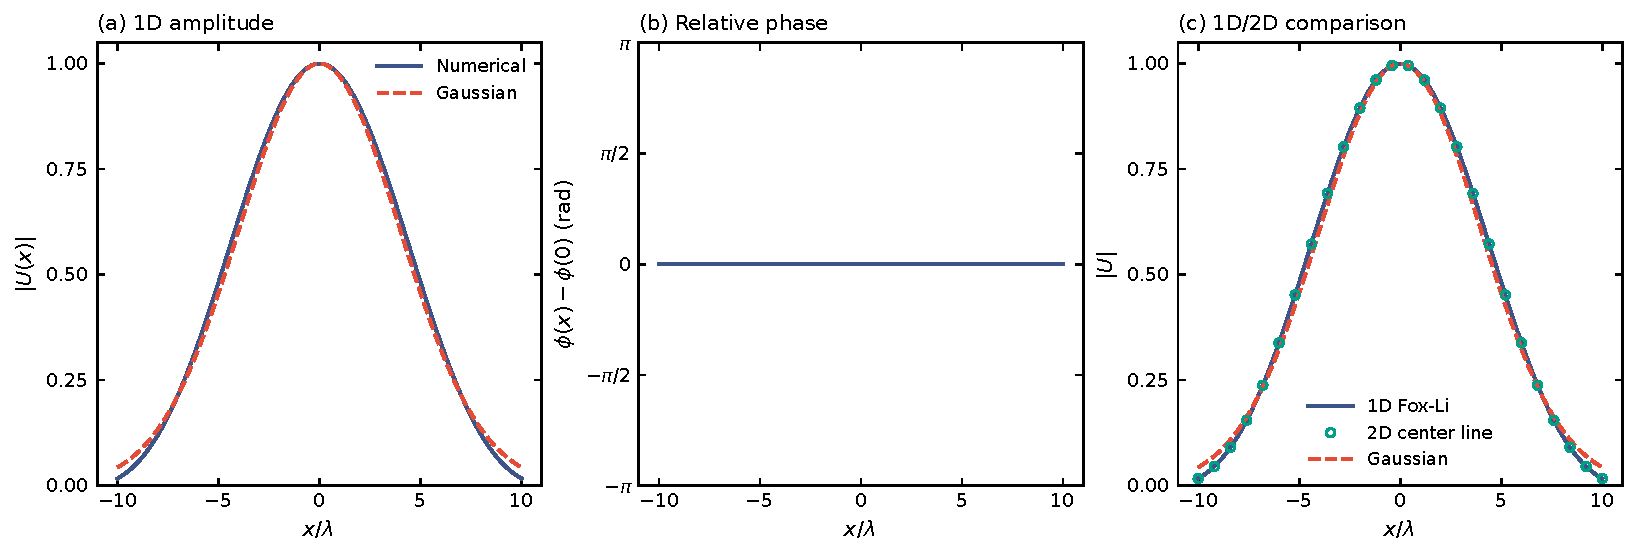
\includegraphics[width=0.98\linewidth]{report_base_validation.pdf}
  \caption{基础自再现模式：(a) 一维振幅与 Gaussian 理论对比；(b) 一维相对中心相位；(c) 一维/二维中心截线比较}
  \label{fig:base-validation}
\end{figure}

数值场的 \(1/e\) 振幅半径约为\(w_{\mathrm{num}}\approx5.8\lambda\),
而对称共焦腔镜面处的理论值为~\cite{xia2016laser,kogelnik1966laser}
\begin{equation}
    w_s=\sqrt{\frac{L\lambda}{\pi}}
    \approx5.642\lambda .
\end{equation}
将该窗口加密采样后，数值 \(1/e\) 半径基本稳定在 \(5.79\lambda\) 附近。
数值自再现模与理想 Gaussian 基模之间仍存在小幅差别。
数值振幅在主要有效场区间内与理论 Gaussian 曲线保持较好一致，
说明当前传播核和 Fox--Li 模式筛选能够正确复现对称共焦腔的低阶自再现模式。

\FloatBarrier
\subsection{收敛过程与本征值}
本征值与自再现残差随迭代次数的变化如图~\ref{fig:convergence} 所示。

\begin{figure}[!htbp]
  \centering
  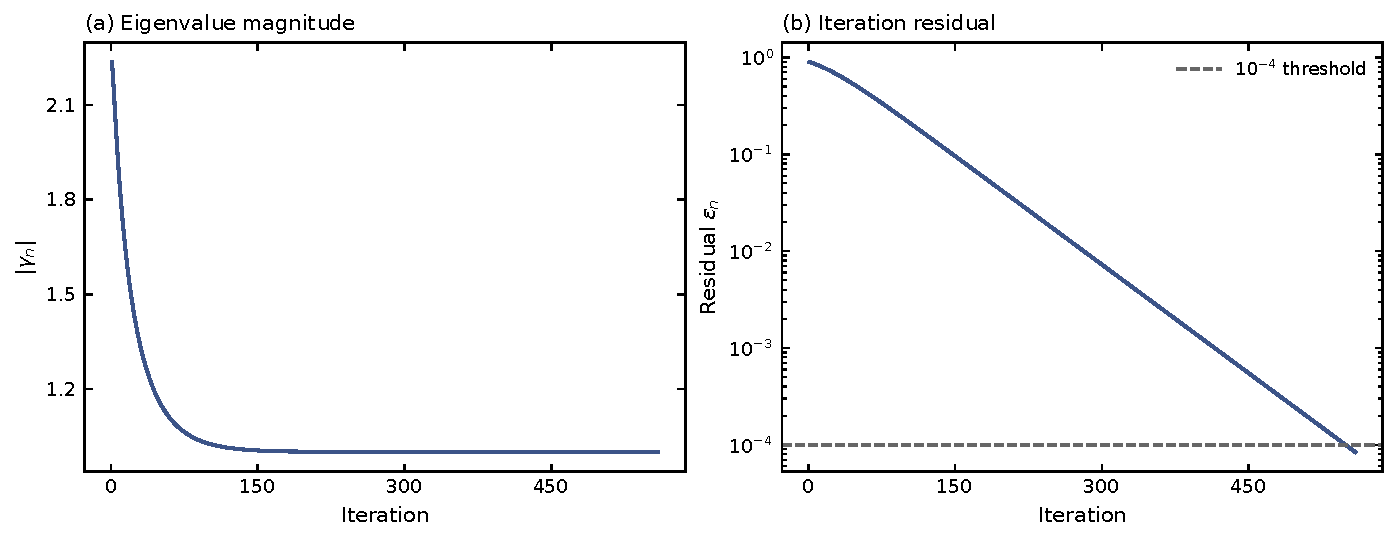
\includegraphics[width=0.92\linewidth]{report_convergence.pdf}
  \caption{基础 Fox--Li 迭代中的本征值幅值与自再现残差收敛过程}
  \label{fig:convergence}
\end{figure}

在当前参数下，基础一维场约在第 559 次迭代后满足“残差连续 10 次低于 \(10^{-4}\)”的停止条件。随着迭代进行，\(|\gamma_n|\) 逐渐趋于稳定，而残差 \(\epsilon_n\) 整体下降并最终进入阈值以下。

最终收敛的本征值幅值为 \(|\gamma|=1.0000221853\)，相位因子为 \(\arg\gamma=-0.785398\,\mathrm{rad}\)。对应的单程功率损耗为
\begin{equation}
    \delta_1=1-\frac{1}{|\gamma|^2}
    \approx4.4369\times10^{-5},
\end{equation}

上述收敛过程体现了 Fox--Li 迭代的模式筛选作用：当不同模式的衍射损耗不同时，初始场中的高损耗成分在反复传播后相对减弱，低损耗成分逐渐占主导，从而形成稳定的自再现模式。

\FloatBarrier
\subsection{二维自再现模式}
基础二维以独立单程迭代在第 579 次满足收敛判据。
对最终场评估，往返残差约为 \(1.41830\times10^{-6}\)。
二维计算结果如图~\ref{fig:base-2d} 所示。归一化振幅在 \(x\) 和 \(y\) 两个方向上均保持中心对称和单峰特征，与对称共焦腔基模应有的横向对称性一致。有效光斑区域内的相位基本保持均匀。

\begin{figure}[!htbp]
  \centering
  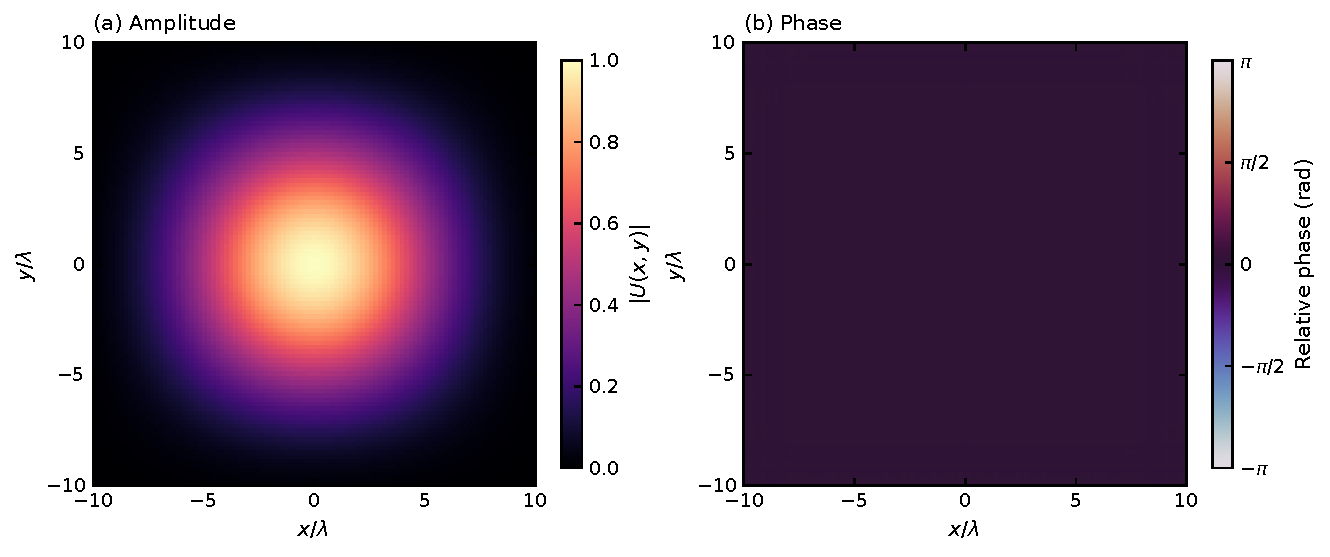
\includegraphics[width=0.86\linewidth]{report_base_2d.pdf}
  \caption{基础二维自再现模式的归一化振幅与相位分布}
  \label{fig:base-2d}
\end{figure}


\FloatBarrier
\subsection{一维与二维一致性}
图~\ref{fig:base-validation}(c) 比较了二维模式的中心截线、一维 Fox--Li 数值结果以及 Gaussian 理论曲线。二维中心截线与一维结果的振幅均方根差约为
\begin{equation}
    E_{\mathrm{1D-2D}}\approx8.69248\times10^{-6}.
\end{equation}
二维中心截线与一维结果高度一致，进一步验证了二维可分离实现。

\subsection{参数选择与数值可靠性}
较大的横向窗口（如 \(a=25\lambda\)）在有限迭代次数内难以筛出理论 Gaussian。为确定合适的横向窗口，比较了不同横向窗口和采样设置下的迭代结果，见表~\ref{tab:window-test}。

\begin{table}[!htbp]
  \centering
  \caption{不同横向窗口与采样设置下的迭代结果}
  \label{tab:window-test}
  \begin{tabular}{cccc}
    \toprule
    \(a/\lambda\) & 网格点数 & \(\Delta x/\lambda\) & 迭代后 \(1/e\) 附近位置 \\
    \midrule
    25 & 101 & 0.5 & 约 \(24\lambda\) \\
    10 & 41  & 0.5 & 约 \(6.0\lambda\) \\
    25 & 251 & 0.2 & 约 \(23.8\lambda\) \\
    10 & 101 & 0.2 & 约 \(5.8\lambda\) \\
    \bottomrule
  \end{tabular}
\end{table}

相同网格间隔下缩小横向窗口后，结果明显接近理论 Gaussian；对过大的窗口，单独加密网格改善有限。因此本文最终采用 \(a=10\lambda\) 作为基础验证参数。

\section{镜面倾斜}
采用第 1 章的线性相位与第 2 章的完整往返模型。倾角扫描使用可分离的一维计算合成二维场，代表场图另作完整二维迭代，两种计算满足同一残差判据且结果一致。

固定其余腔参数，在 \(0\leq\theta\leq0.05\,\mathrm{rad}\) 范围内扫描倾角，步长为 \(0.005\,\mathrm{rad}\)，考察自再现模式及其特征量随倾角的变化。

\subsection{倾角增大过程中的二维模场变化}
为直观展示模式随倾角增大的变化，选取\(\theta=0\)、\(0.025\) 和 \(0.05\,\mathrm{rad}\) 三个代表角度进行二维计算，结果如图~\ref{fig:tilt-2d} 所示。

\begin{figure}[!htbp]
  \centering
  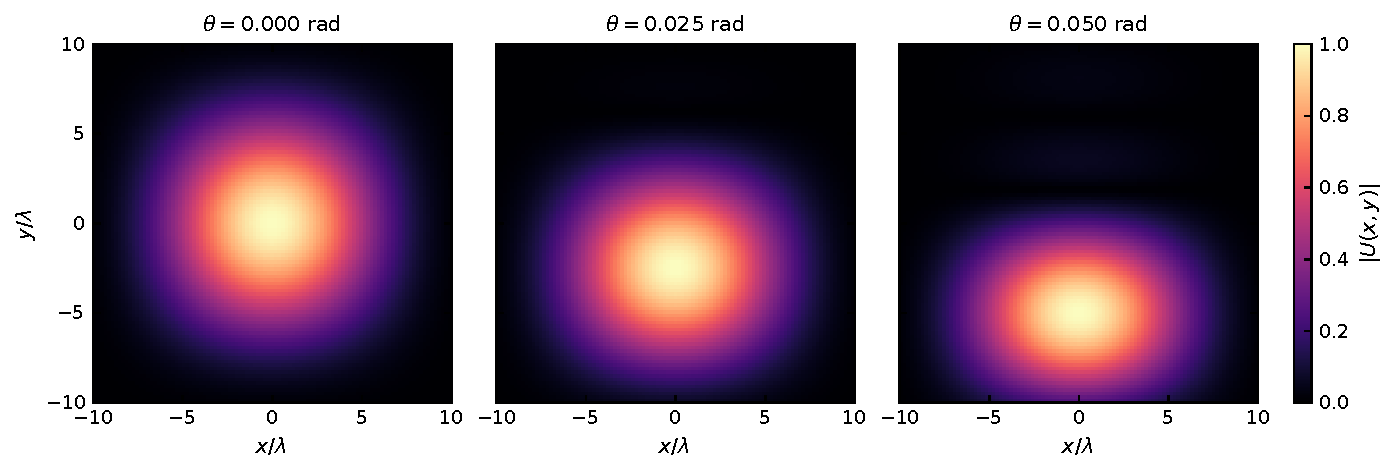
\includegraphics[width=0.92\linewidth]{report_tilt_2d.pdf}
  \caption{不同镜面倾角下的二维自再现模式振幅分布}
  \label{fig:tilt-2d}
\end{figure}

在 \(\theta=0\) 时，模式中心位于坐标原点附近；当倾角增加到 \(0.025\,\mathrm{rad}\) 和 \(0.05\,\mathrm{rad}\) 时，二维模式中心分别移动到约 \(-2.50\lambda\) 和 \(-5.00\lambda\)。受扰动的 \(y\) 方向模宽明显减小，而未受扰动的 \(x\) 方向模宽始终保持在约 \(5.67\lambda\) 附近。

图中所示的二维场保持单峰，未出现明显的新节线或多瓣结构，主要表现为模式的偏移和形变。

\FloatBarrier
\subsection{模式特征量随倾角的变化}
中心位置、两个方向的模半径、往返损耗和本征值幅值的主要结果汇总于图~\ref{fig:tilt-quantitative}。

\begin{figure}[H]
  \centering
  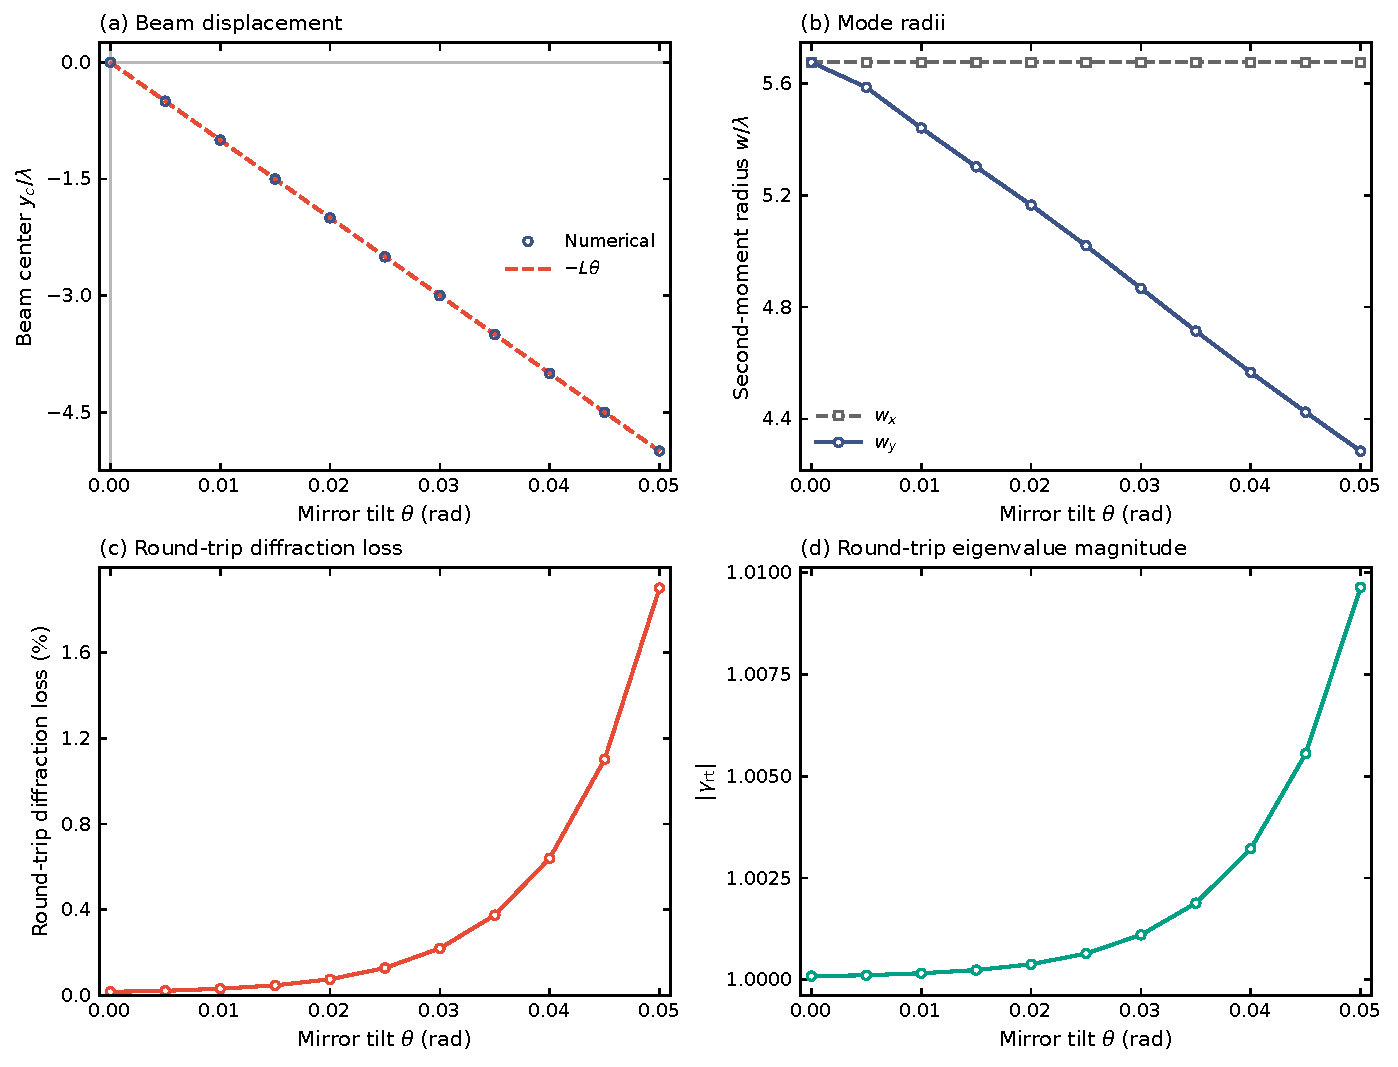
\includegraphics[width=0.94\linewidth]{report_tilt_quantitative.pdf}
  \caption{镜面倾角对光束中心、两个方向的二阶矩模半径、完整二维往返功率损耗及本征值幅值的影响}
  \label{fig:tilt-quantitative}
\end{figure}

\subsubsection{光束中心}
如图~\ref{fig:tilt-quantitative}(a) 所示，在所扫描的正倾角范围内，模式中心沿负 \(y\) 方向近似线性移动，数值结果与 \(-L\theta\) 参考线接近。

为进一步检验小角度下的线性关系，在 \(-0.01\leq\theta\leq0.01\,\mathrm{rad}\) 区间内按 \(0.001\,\mathrm{rad}\) 的步长进行 21 点对称扫描。对小角度区间内的数值中心进行线性拟合，得到\(\frac{\mathrm{d}y_c}{\mathrm{d}\theta} \approx-99.9888\lambda/\mathrm{rad}\)。
由于当前腔长为 \(L=100\lambda\)，拟合斜率与 \(-L\) 基本一致，因此在当前小角度范围内可以写成
\begin{equation}
    y_c\approx-L\theta .
\end{equation}
相对于该线性关系，上述小角度扫描区间内的最大绝对偏差约为\(2.17344\times10^{-4}\lambda\)。

\subsubsection{模半径}
如图~\ref{fig:tilt-quantitative}(b) 所示，倾斜方向的二阶矩模半径随倾角增大而逐渐减小，从 \(\theta=0\) 时约\(w_y\approx5.676\lambda\)
减小到 \(\theta=0.05\,\mathrm{rad}\) 时约\(w_y\approx4.285\lambda\)。未受扰动的 \(x\) 方向二阶矩模半径基本保持在约 \(5.676\lambda\) 附近，与二维场图中两个方向模宽的变化一致。

\subsubsection{往返损耗与本征值}
如图~\ref{fig:tilt-quantitative}(c) 所示，完整二维往返功率损耗同样随倾角明显增加。无倾斜时\(D \approx1.78\times10^{-4}\),
而当 \(\theta=0.05\,\mathrm{rad}\) 时增大到\(D \approx1.90\times10^{-2}\),
即约 \(1.90\%\)。在小倾角附近损耗增长相对缓慢，而随着模式中心逐渐远离腔轴，有限孔径对模式的影响增强，往返衍射损耗开始明显上升。该趋势与二维场图中模式逐渐靠近孔径边缘的现象一致。

由 \(D=1-1/|\gamma_{\mathrm{rt}}|^2\)，完整二维往返本征值幅值为 \(|\gamma_{\mathrm{rt}}|=1/\sqrt{1-D}\)。
如图~\ref{fig:tilt-quantitative}(d) 所示，随着倾角由 0 增至 \(0.05\,\mathrm{rad}\)，其幅值由 \(1.00008888\) 增大至 \(1.00963916\)。\(|\gamma_{\mathrm{rt}}|\) 增大意味着传播后的振幅比例 \(1/|\gamma_{\mathrm{rt}}|\) 减小，与往返损耗增加相一致。

\FloatBarrier
\subsection{物理解释}
镜面倾斜在反射时引入与 \(y\) 成线性关系的附加相位，相当于改变了场的横向相位梯度。该相位梯度在后续传播过程中转化为横向位置偏移，因此模式中心随倾角近似线性移动。在小角度和当前共焦参数下，所得 \(y_c\approx-L\theta\) 的数值关系表明这一传播过程与简单几何量级相符。

当倾角继续增大时，模式中心逐渐靠近有限孔径边缘，腔内能够稳定自再现的场分布需要重新调整。在当前有限孔径和共焦参数下，数值结果表现为倾斜方向模宽减小，同时边缘截断相关的往返衍射损耗显著增加。这说明镜面失调的影响不仅体现在光束中心位置，还会改变稳定模式的横向尺度和损耗。

\Needspace{0.75\textheight}
\section{镜面局部凸起}

\subsection{自再现条件与典型模场}
采用式~\eqref{eq:hemisphere} 的半球模型，默认从均匀场出发，作完整往返迭代。图~\ref{fig:bump-mode} 比较无扰动、中心 \(r_b=2\lambda\) 和离轴 \(r_b=2\lambda,P=(6\lambda,0)\) 的场分布。
\begin{figure}[H]
 \centering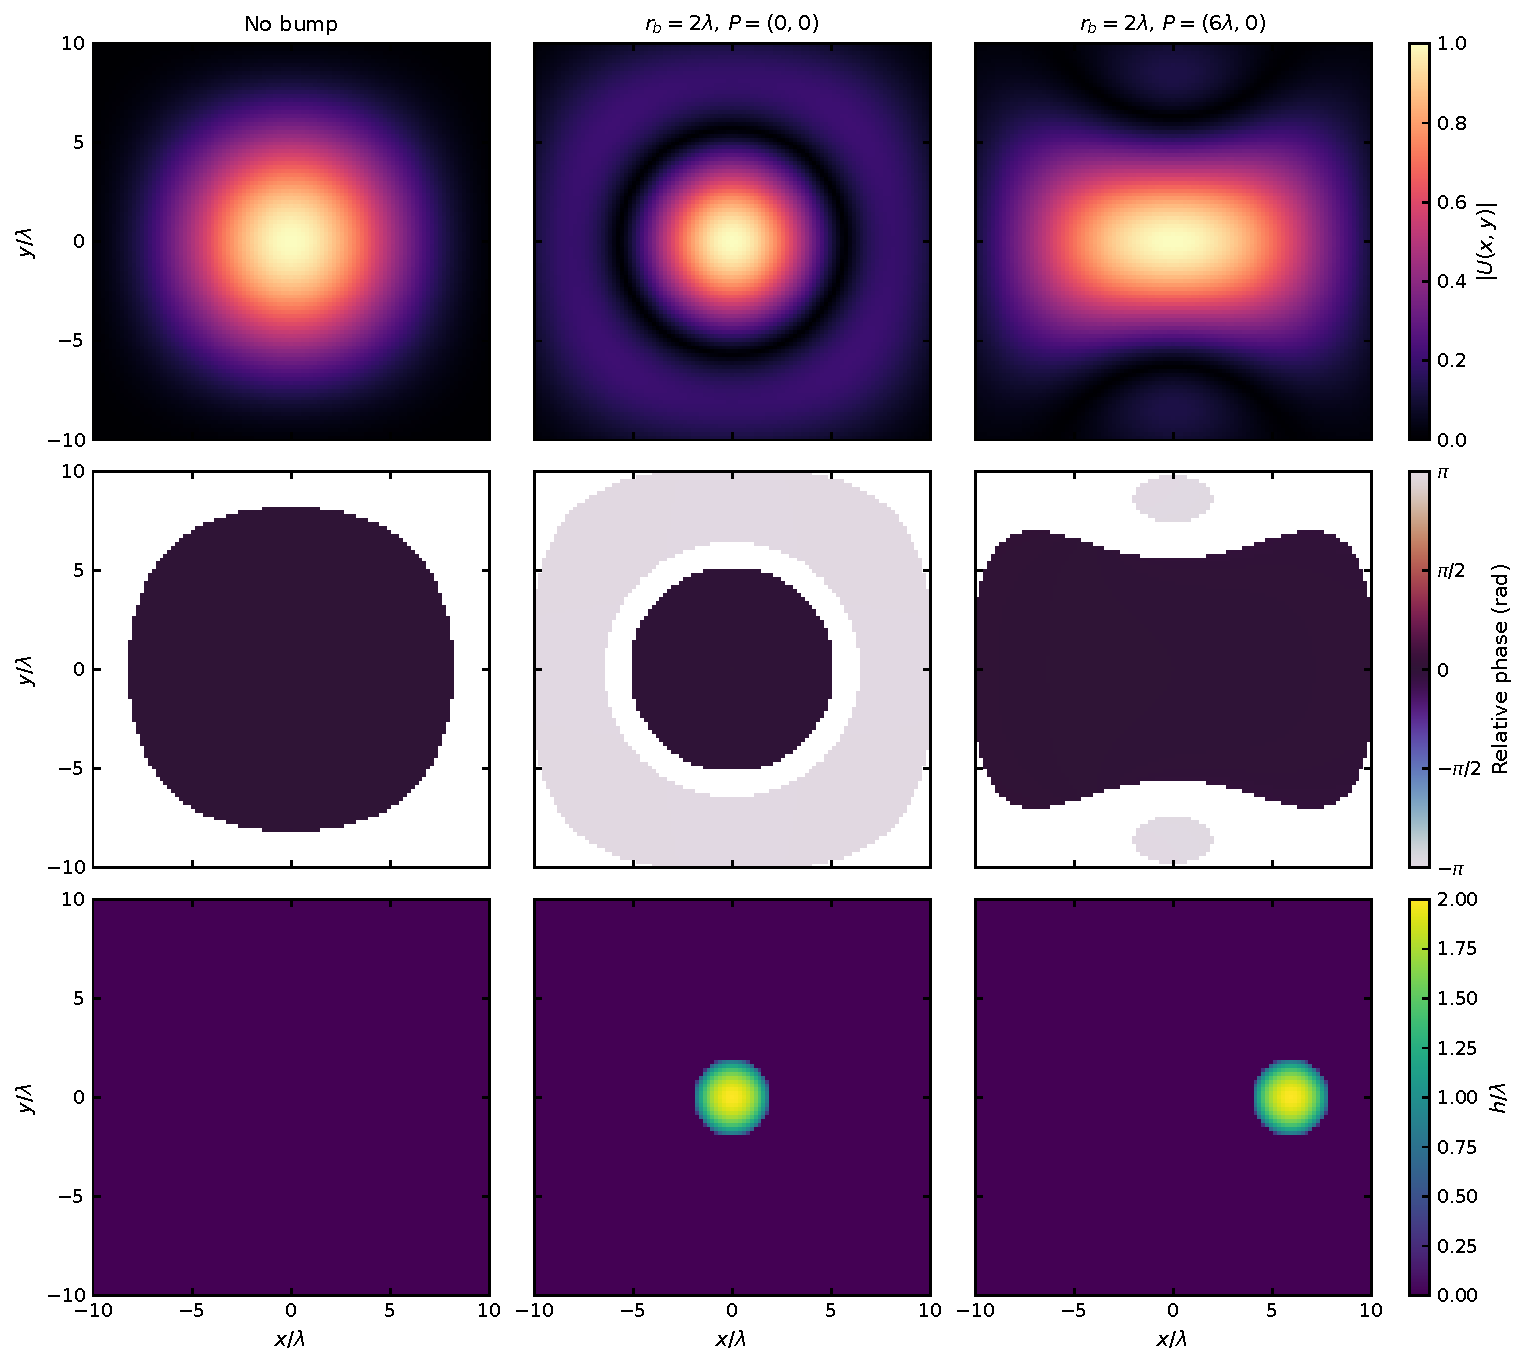
\includegraphics[width=0.98\linewidth]{bump_mode.pdf}
 \caption{无扰动、中心半球凸起与离轴半球凸起的二维振幅、相对相位和镜面形貌}\label{fig:bump-mode}
\end{figure}
中心凸起改变光斑内部的反射相位，形成明显的环状节点和模场畸变；离轴凸起破坏原有对称性，模式不再只是理想场的平移。

\FloatBarrier
收敛过程见图~\ref{fig:bump-convergence}。无扰动、中心 \(r_b=2\lambda\)、离轴 \(P=(6\lambda,0)\) 分别在 176、137、246 次往返后满足停止条件，说明所选参数下均存在稳定的自再现模式。
\begin{figure}[!htbp]
 \centering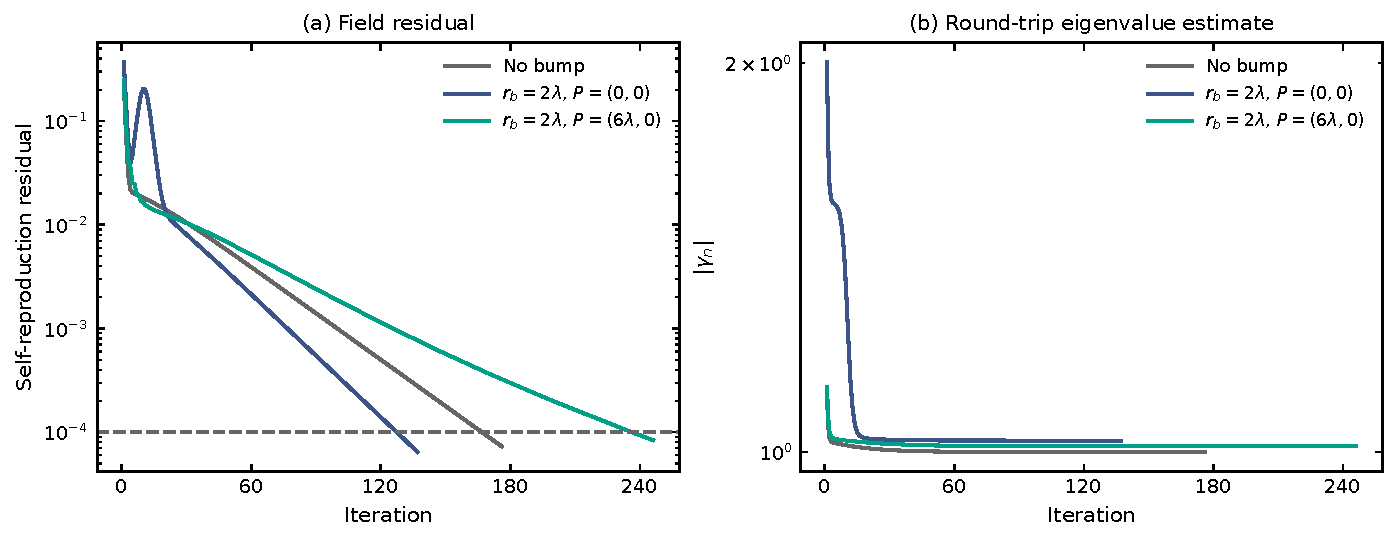
\includegraphics[width=0.97\linewidth]{bump_convergence.pdf}
 \caption{半球凸起计算中的场残差与往返本征值估计}\label{fig:bump-convergence}
\end{figure}

\FloatBarrier
\subsection{凸起半径的影响}
保持中心 \(P=(0,0)\)，扫描 \(r_b=0,1,2,3,4\lambda\)，结果见图~\ref{fig:bump-radius}。全部五点均满足残差判据；半径增大时，总往返损耗总体上升，模式与无扰动参考场的重叠度降低。
\begin{figure}[H]
 \centering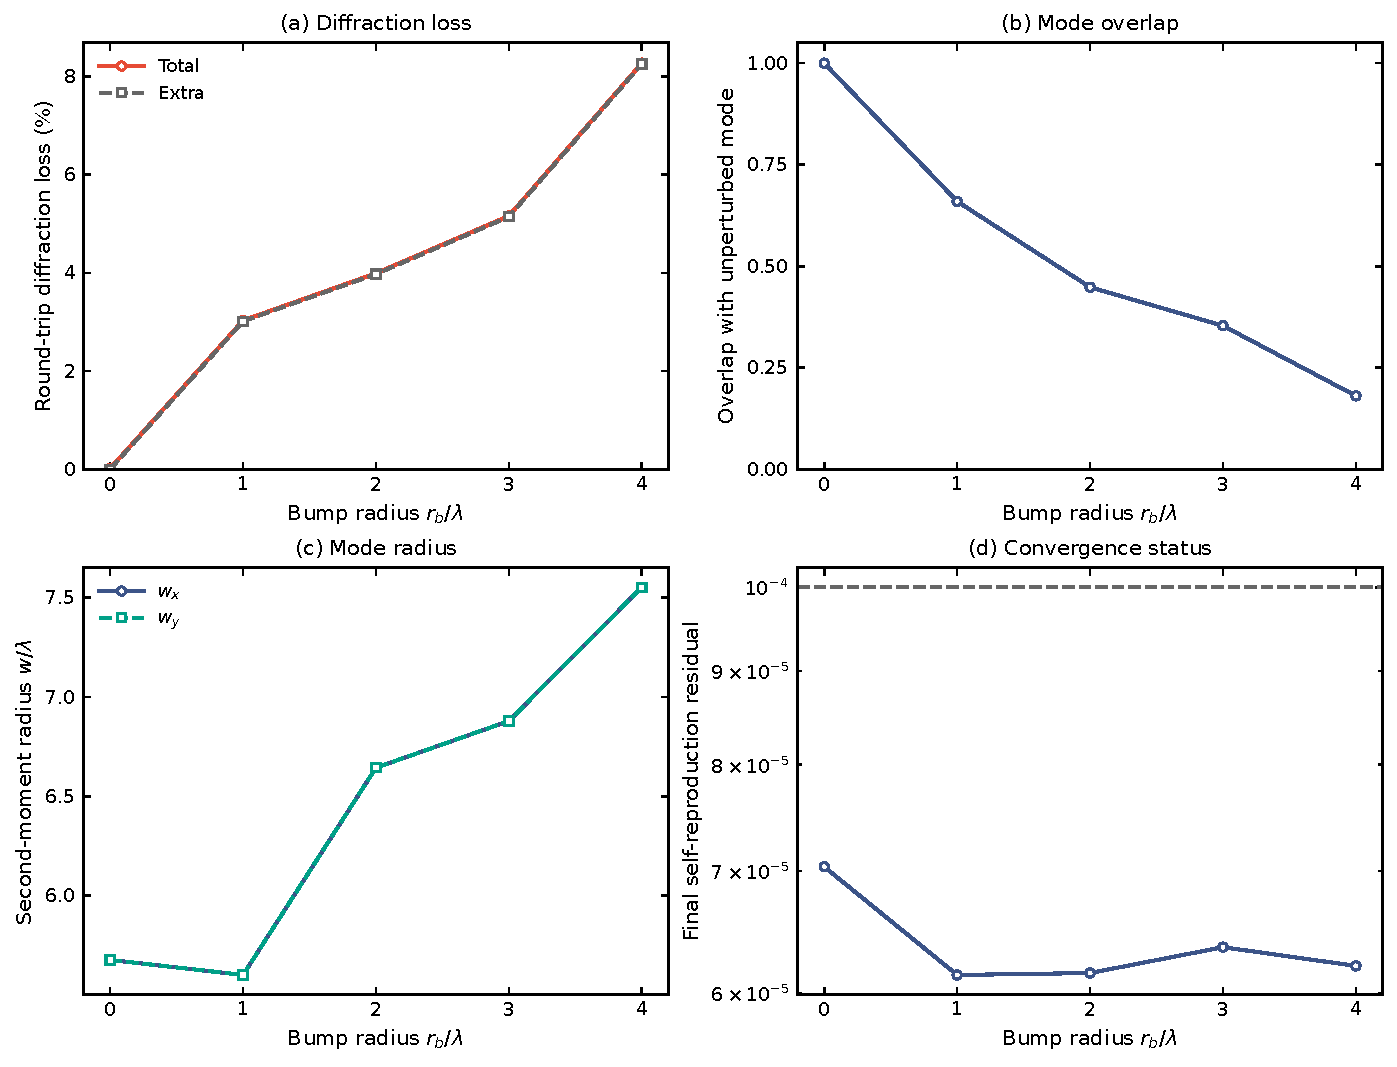
\includegraphics[width=0.96\linewidth]{bump_radius.pdf}
 \caption{中心半球凸起半径对往返损耗、模式重叠度、二阶矩半径及收敛残差的影响}\label{fig:bump-radius}
\end{figure}
\(r_b=1,2,4\lambda\) 时，总往返损耗分别约为 3.033\%、3.993\%、8.273\%，重叠度分别约为 0.660、0.448、0.181。半球半径同时改变高度和横向覆盖范围，因此该扫描反映的是两者的综合影响。

\FloatBarrier
\subsection{凸起位置的影响}
固定 \(r_b=2\lambda,y_c=0\)，沿 \(x_c=0,1,2,4,6\lambda\) 扫描，结果见图~\ref{fig:bump-position}。\(x_c=1,2,4\lambda\) 的收敛场与基模重叠度接近 0，场型发生明显变化；\(x_c=6\lambda\) 时重叠度约为 0.874，总损耗约 2.023\%，明显比中心凸起更接近参考模式。这表明凸起靠近光斑中心区域时会显著改变所选模式，而移到光斑边缘附近后影响明显减弱。
\begin{figure}[!htbp]
 \centering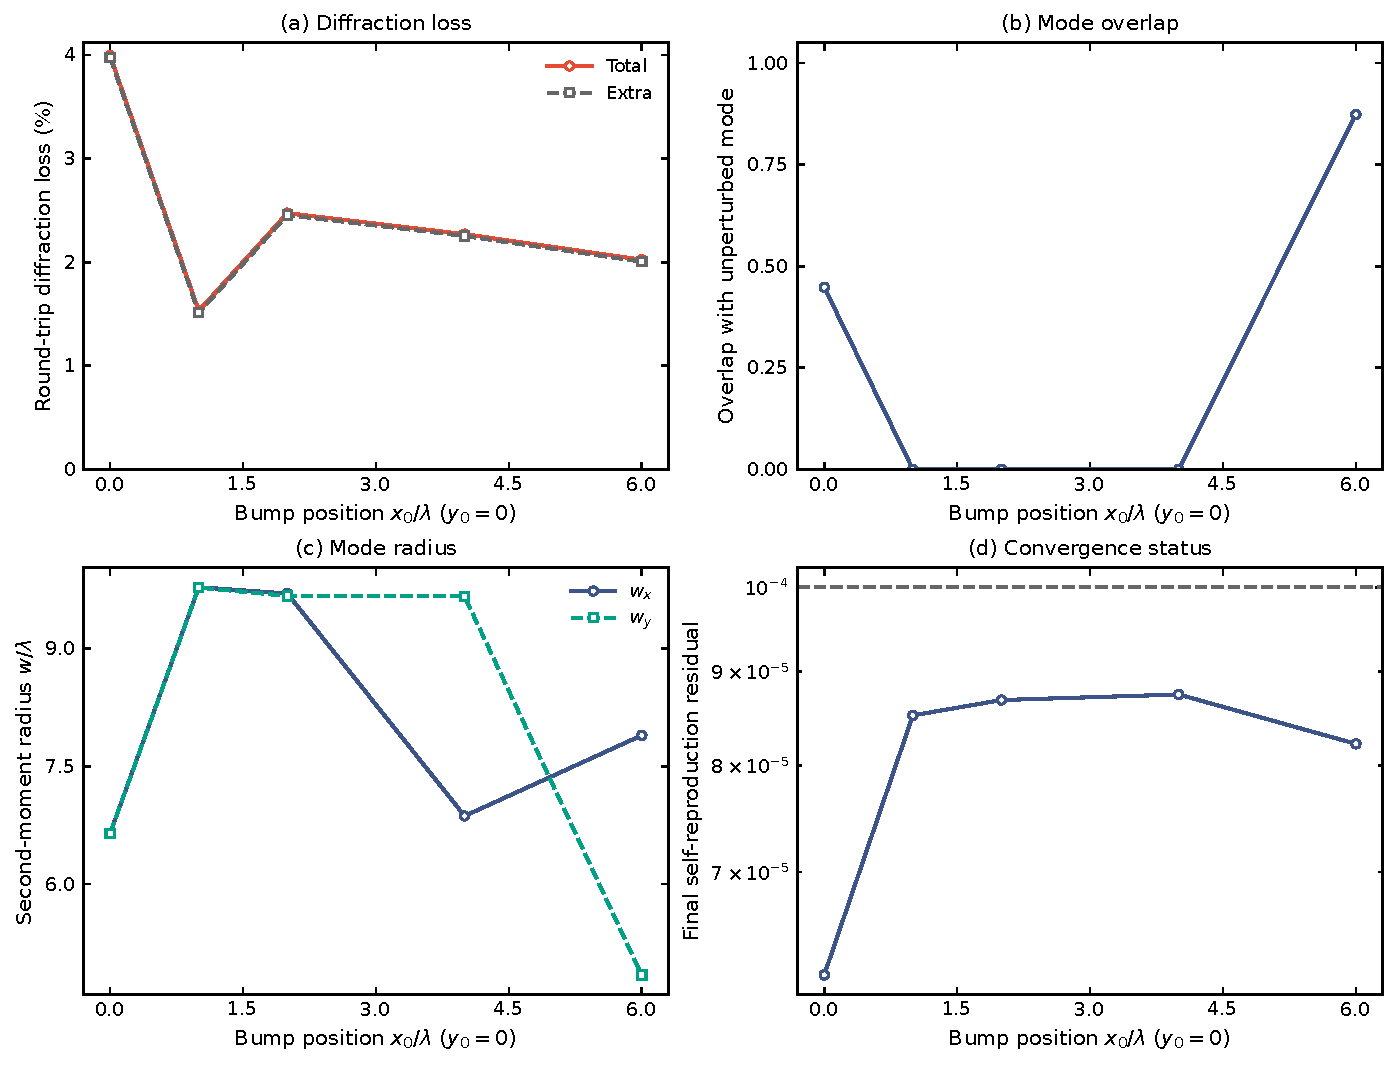
\includegraphics[width=0.96\linewidth]{bump_position.pdf}
 \caption{半球凸起位置扫描}\label{fig:bump-position}
\end{figure}

\FloatBarrier
\subsection{物理解释}
半球凸起在光斑强区引入局部非均匀反射相位，使往返场重新选模，表现为环状节点、场型畸变和附加衍射损耗。凸起半径增大时，高度和横向覆盖范围同时增加，扰动增强；凸起移出光斑主区后，其覆盖范围内场强很低，对模式的影响随之减小。

\clearpage
\section*{结论}
\markboth{结论}{结论}
\addcontentsline{toc}{section}{结论}
本文建立了一维与二维共焦腔 Fox--Li 计算，并在相同网格、传播核和正常镜面上研究单镜倾斜与半球凸起。基础模式的最近采样点 \(1/e\) 振幅半径约为 \(5.8\lambda\)，理论镜面半径为 \(5.642\lambda\)；一维与二维中心截线 RMS 差约 \(8.69248\times10^{-6}\)，基础模式与理论低阶模式较接近。

两种扰动都通过反射相位改变往返模式，但表现不同：倾斜是沿 \(y\) 的线性相位，
主要造成中心偏移，在小角范围内有 \(y_c\approx-L\theta\)，
较大倾角伴随模宽和衍射损耗变化；半球凸起是局部非均匀相位，
会造成节点、畸变以及位置相关的模式筛选。表~\ref{tab:mirror-comparison}
用同一无扰动完整往返场作为基准，对比扰动结果。

\begin{table}[!htbp]
 \centering\small
 \caption{两类镜面扰动的代表结果}\label{tab:mirror-comparison}
 \begin{tabular}{lrrr}\toprule
 扰动参数 & 总损耗（\%） & 附加损耗（百分点） & 重叠度\\\midrule
 无扰动 & 0.017773 & 0 & 1.000000\\
 倾斜 \(\theta=0.005\,\mathrm{rad}\) & 0.022230 & 0.004457 & 0.991863\\
 倾斜 \(\theta=0.025\,\mathrm{rad}\) & 0.128849 & 0.111077 & 0.790177\\
 倾斜 \(\theta=0.05\,\mathrm{rad}\) & 1.900326 & 1.882553 & 0.315601\\
 中心半球 \(r_b=1\lambda\) & 3.032773 & 3.015000 & 0.659607\\
 中心半球 \(r_b=2\lambda\) & 3.993419 & 3.975646 & 0.448391\\
 中心半球 \(r_b=4\lambda\) & 8.273023 & 8.255250 & 0.180961\\
 离轴半球 \(r_b=2\lambda,P=(6\lambda,0)\) & 2.023081 & 2.005308 & 0.873721\\
 \bottomrule\end{tabular}
\end{table}

综上所述，Fox--Li 迭代能够正确描述自再现模式及镜面扰动的趋势。

\clearpage
\begingroup
\ctexset{subsection={beforeskip=4pt,afterskip=2pt}}
\section*{附录 A：AI 辅助过程、客观评价与本人工作}
\markboth{附录 A}{附录 A}
\addcontentsline{toc}{section}{附录 A：AI 辅助过程、客观评价与本人工作}

\subsection*{AI 辅助的具体案例}
第一个案例是本征值估计异常。基础场型在约 300 次迭代后未见明显变化，但逐点相除再平均得到的 \(|\gamma|\) 仍有明显波动。AI 帮助分析了弱场小分母对等权平均的影响，并提出整体最小二乘估计作为候选方法。通过比较新旧方法的迭代曲线和最终值、检查不同位置的传播比例、进行带中心节点的场测试并检查自再现残差，最终采用式~\eqref{eq:gamma} 估计本征值，以全场残差判断收敛。

第二个案例是倾斜腔计算的性能优化。加入完整往返传播后，运行时间显著增加，计时和代码检查定位到传播核在每次调用中被重复计算。AI 帮助分析了固定网格、腔长和曲率下传播核的复用条件，以及预计算 \(K\) 后使用矩阵乘法与原离散积分的对应关系。修改后，对照优化前后的模式中心、残差和运行时间，最终采用传播核预计算。单次传播由约 \(0.010\,\mathrm{s}\) 降至约 \(2.7\times10^{-4}\,\mathrm{s}\)，完整无界面测试由约 \(96\,\mathrm{s}\) 降至约 \(1.6\,\mathrm{s}\)。

第三个案例是交互演示程序的开发与优化权衡。为便于验证计算结果和展示物理现象，AI 协助完成演示程序。AI 根据功能需求生成了基于 Tkinter 的多标签页布局框架，包括控件布局、Matplotlib 画布嵌入、以及多线程计算避免界面卡顿的基本结构。该框架代码约 600 行，本人在此基础上补充了物理计算函数的调用、参数验证逻辑、以及与正式计算模块（\texttt{base.py}、\texttt{tilt.py}、\texttt{bump.py}）的接口适配。

在开发过程中，AI 提出了项优化建议：向量化 \texttt{make\_kernel} 函数：
声称可将核函数构建时间从约 \(0.5\,\mathrm{s}\) 降至约 \(0.02\,\mathrm{s}\)，
提速约 25 倍。经测试确实有效，但最终未采纳。
原因：核函数仅预计算一次，优化后对总体运行时间影响可忽略；循环直接对应物理公式中"镜面点到镜面点"的传播关系，代码可读性更强，更符合正式计算模块的设计原则。

该案例体现了 AI 建议需要结合实际场景进行评估，而非盲目采纳。

\subsection*{AI 辅助的作用与评价}
在本征值估计中，AI 帮助分析了弱场小分母引起的比值波动；在性能优化中，AI 帮助梳理了固定传播核的复用条件。本文通过新旧估计方法的迭代曲线、优化前后的模场与残差对照，以及运行时间测试，检查修改效果。

\subsection*{本人完成的工作}
本人完成了三类工作：

1.物理建模与参数设置，包括根据教材建立对称共焦腔模型、
单镜倾斜的完整往返模型，以及设置窗口、网格、倾角范围和中心、模宽、损耗等指标。

2.程序实现与实验验证，包括一维离散传播、二维可分离传播、归一化、本征值估计和收敛判断，
以及 Gaussian 理论对比、窗口和网格控制实验、传播核预计算和优化前后交叉验证；代码编写和测试由本人完成。

3.结果分析与交付整理，包括二维倾斜结果分析、参数扫描、报告图生成，以及交互 Demo 的功能设计、
测试与整理。

\endgroup
\clearpage
\section*{附录 B：程序与复现说明}
\markboth{附录 B 与参考文献}{附录 B 与参考文献}
\addcontentsline{toc}{section}{附录 B：程序与复现说明}
源码位于 \texttt{src/}，
图像与原始结果位于 \texttt{figures/} 和 \texttt{figures/data/}，
报告源文件位于 \texttt{latex/}。
基础、倾斜、凸起分别由 \texttt{base.py}、\texttt{tilt.py}、\texttt{bump.py} 计算，绘图与数据整理使用已有脚本。
交互演示入口为根目录的 \texttt{FoxLiDemo.exe}，
包含基础模式、收敛、倾斜、局部凸起和参数扫描页面。
完整环境、参数和编译步骤见随附运行说明。

\bibliographystyle{unsrt}
\bibliography{references}
\markboth{附录 B 与参考文献}{附录 B 与参考文献}
\end{document}
